\section{RISE}
Like LIME, RISE is a block box method and works on manipulation of the input images. Instead of using superpixels, RISE generates masks that are then applied to the input images by multiplying the mask with the input image pixel values. Figure \ref{rise_mask0} and Figure \ref{rise_mask1} show two RISE masks applied to the same input image.

\begin{figure}[H]
    \centering
    \begin{subfigure}[t]{.32\textwidth}
        \centering
        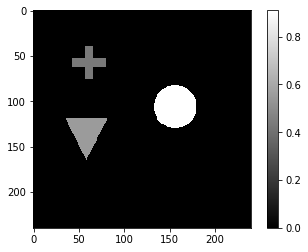
\includegraphics[width=\linewidth]{chapters/02_methods/images/rise/rise_original.png}
        \caption{Original image}
    \end{subfigure}\hfill%
    \begin{subfigure}[t]{.32\textwidth}
        \centering
        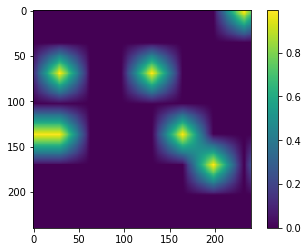
\includegraphics[width=\linewidth]{chapters/02_methods/images/rise/rise0_mask.png}
        \caption{RISE mask}
    \end{subfigure}\hfill%
    \begin{subfigure}[t]{.32\textwidth}
        \centering
        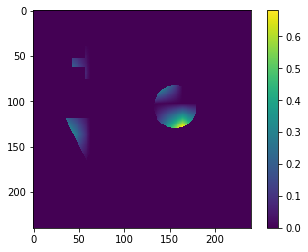
\includegraphics[width=\linewidth]{chapters/02_methods/images/rise/rise0_applied.png}
        \caption{RISE mask applied to original image by multiplication}
    \end{subfigure}
    \caption{By multiplication the input image (left) with a RISE mask (center), a modified input is generated.}
    \label{rise_mask0}
\end{figure}


\begin{figure}[H]
    \centering
    \begin{subfigure}[t]{.32\textwidth}
        \centering
        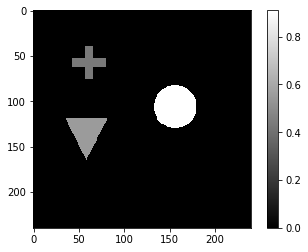
\includegraphics[width=\linewidth]{chapters/02_methods/images/rise/rise_original.png}
        \caption{Original image}
    \end{subfigure}\hfill%
    \begin{subfigure}[t]{.32\textwidth}
        \centering
        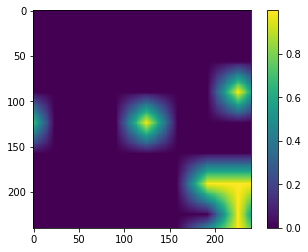
\includegraphics[width=\linewidth]{chapters/02_methods/images/rise/rise1_mask.png}
        \caption{RISE mask}
    \end{subfigure}\hfill%
    \begin{subfigure}[t]{.32\textwidth}
        \centering
        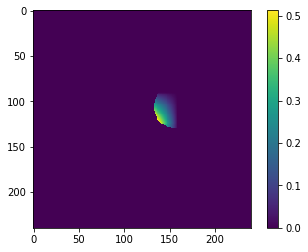
\includegraphics[width=\linewidth]{chapters/02_methods/images/rise/rise1_applied.png}
        \caption{RISE mask applied to original image by multiplication}
    \end{subfigure}
    \caption{By multiplication the input image (left) with a RISE mask (center), a modified input is generated. In comparison fo Figure \ref{rise_mask0}, this input image retains much less information.}
    \label{rise_mask1}
\end{figure}


TODO: matrix multiplication

To visualize the generated explanation map, the data is upscaled to the original image size and displayed as a heatmat by mapping the values to a color map. Figure \ref{rise_example} show some examples for visualization of the RISE output for specific classes.

\begin{figure}[H]
\centering
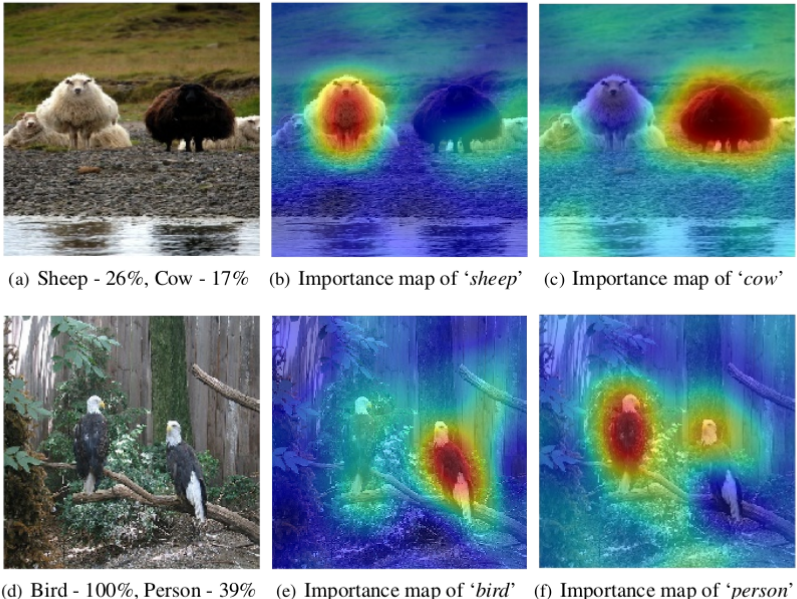
\includegraphics[width=12cm]{chapters/02_methods/images/rise/sheep.png}
\caption{Image from original paper explaining some classes}
\label{rise_example}
\end{figure}
